\documentclass[16pt]{beamer}
\usecolortheme{dolphin}

\usepackage[orientation=landscape,size=custom,width=117,height=85,scale=1]{beamerposter}
\usepackage[absolute,overlay]{textpos}
\usepackage{amsmath}
\usepackage{amsthm}
\usepackage{framed}
\usepackage{array}

\newtheorem{conjecture}[theorem]{Conjecture}

\renewcommand{\arraystretch}{1.4}
\newcommand{\Q}{\mathbb{Q}}
\newcommand{\Z}{\mathbb{Z}}
\newcommand{\N}{\mathbb{N}}
\newcommand{\R}{\mathbb{R}}
\newcommand{\C}{\mathbb{C}}
\newcommand{\F}{\mathbb{F}}
\newcommand{\Qhat}{\widehat{Q}^{n}(t)}
\newcommand{\What}{\widehat{W}^{n}(t)}
\newcommand{\Qtild}{\widetilde{Q}^{n}(t)}
\newcommand{\Qfhat}{\widehat{Q}^{n}(\cdot)}
\newcommand{\Wfhat}{\widehat{W}^{n}(\cdot)}
\newcommand{\Qftild}{\widetilde{Q}^{n}(\cdot)}
\newcommand{\error}{E^{n}(\cdot)}

\setlength{\TPHorizModule}{1cm}
\setlength{\TPVertModule}{1cm}


\begin{document}

\setbeamertemplate{frametitle}[default][center]
\begin{frame}
\frametitle{\\ {\Huge Investigating the Effect of Variance in Markovian Shortest Remaining Processing Time Queues}\\  Sean Malter and Dr. Amber Puha, Department of Mathematics, California State University, San Marcos}










\begin{textblock}{35}(2,7)
\begin{block}{\huge Queues and Service Disciplines}
A queue can be thought of as a waiting line, with jobs waiting to be served and jobs in service. The order in which we process the jobs in the queue is called a service discipline.
\vspace{\baselineskip}

\begin{minipage}{18cm}
First-Come-First-Serve (FCFS)
{\small
\begin{itemize}
\item Jobs served one at time in order of arrival
\item Oldest job gets all of the sever's effort
\item Typical for serving people, e.g., at a small retail store with one cash register
\end{itemize}
}
\vspace{0.5cm}
Processor Sharing (PS)
{\small
\begin{itemize}
\item Serves jobs all jobs simultaneously
\item Servers effort is divided equal among all jobs
\item Idealized computer time sharing
\end{itemize}
}
\vspace{0.5cm}
Shortest Remaining Processing Time (SRPT)
{\small
\begin{itemize}
\item Job with the smallest remaining processing time served first
\item Preemptive (the new job with a smaller
processing time than the remaining processing time of the job in service gets priority)
\item Performance Optimal: Known to minimizes queue length
\end{itemize}
}
\end{minipage}
\begin{minipage}{16cm}
\begin{center}

\includegraphics[width=16cm]{Pictures/queue.jpg}
\end{center}
\end{minipage}
\end{block}
\vspace{\baselineskip}

\begin{block}{\huge Heavily Loaded M/M/1 Queue}
Interarrival times and processing times are sequences of mutually independent, independent exponential random variables with respective rates ${\color{orange}\lambda}$ and ${\color{orange}\mu}$. 

 We investigate heavily loaded M/M/1 queues where ${\color{orange}\mu=\lambda}$.
\vspace{\baselineskip}
\end{block}

\begin{block}{\huge Performance Processes}
%\vspace{\baselineskip}
\begin{itemize}
\item \textbf{Queue Length}: {\color{green}$Q(t)$}, the number of jobs in the system at time $t$
\item \textbf{Workload}: {\color{red}$W(t)$}, the total time needed to complete all the work in the system at time $t$, excluding future arrivals.
\end{itemize}
\vspace{\baselineskip}
\end{block}

\begin{block}{\huge Natural Question}
Can one quantify how small the queue length process is for an SRPT queue?
\vspace{\baselineskip}
\end{block}

\begin{block}{\huge An Answer Under Standard Diffusion Scaling}
For $n\in{\mathbb N}$ and $t \in [0,\infty)$,
\[
{\color{red}\widehat{W}^{n}(t) = \frac{W(nt)}{\sqrt{n}}}
\quad\hbox{and}\qquad
{\color{green}\widehat{Q}^{n}(t) = \frac{Q(nt) } {\sqrt{n}}}.
\]
\vspace{\baselineskip}
Established SRPT convergence in distribution results: as $n\to\infty$
\[
{\color{red}\widehat{W}^{n}(\cdot)\Rightarrow W^*(\cdot)}
\qquad\hbox{and}\qquad
{\color{green}\widehat{Q}^{n}(\cdot)\Rightarrow 0}.
\]
Here  ${\color{red}W^{*}(\cdot)}$ is reflected Brownian motion with variance $2/{\color{orange}\lambda}^2$.\\

{\bf Conlusion:} The queue length process is of smaller order of magnitude than the workload process.
\vspace{\baselineskip}
\end{block}

\begin{block}{\huge Next Natural Question and Suspected Answer}
What is the order of magnitude of the queue length process?\\
We conjecture a correction factor of ${\color{green}\ln(\sqrt{n})}$.\\
We investigated this through simulation.
\vspace{\baselineskip}
\end{block}

\begin{block}{\huge Non-Standard Diffusion Scaling}
For $n\in{\mathbb N}$ and $t\in[0,\infty)$, set
\[
{\color{green}\widetilde{Q}^{n}(t) = \frac{\ln (\sqrt{n}) Q(nt) } {\sqrt{n}}}.
\]
\vspace{\baselineskip}
\end{block}
\begin{block}{\huge Suspected Behavior}
There exists a positive constant ${\color{orange}C}$, depending on ${\color{orange}\lambda}$, such that 
\vspace{\baselineskip}
\[
{\color{orange}C} {\color{red}\Wfhat} \approx {\color{green}\Qftild}, \qquad \text{as } n \rightarrow \infty.
\]
We used simulations to identify a candidate for ${\color{orange}C}$ and to explore viability.
\end{block}
\end{textblock}



\begin{textblock}{35}(41,7)
\begin{block}{\huge Main Outcome}
As a result of our investigation, we developed a conjecture:
\begin{framed}
\begin{conjecture} [Hunsperger, Malter, Puha]
In an M/M/1 SRPT queue with common processing and incoming rate given by ${\color{orange}\lambda}$,
the queue length process appropriately rescaled with a non-standard logarithmic growth
factor converges in distribution to a reflected Brownian motion, i.e.,
${\color{green}\widetilde{Q}^{n}(\cdot)} \Rightarrow {\color{orange}\lambda}{\color{red} W^{*}(\cdot)}$, as  $n \rightarrow \infty$.
\end{conjecture}
\end{framed}
\end{block}

\begin{block}{\huge Identifying the Constant \emph{{\color{orange}C}}}
The following ratio is a natural estimator for $1/{\color{orange}C}$:
\[
\frac{{\color{red}\Wfhat}}{{\color{green}\Qftild}}
\]
Plots of the ratio with $n=10^7$, and$t \in [0, 1/\lambda]$, with values of $t$ for which
${\color{green}\Qtild(t)} = 0$ omitted.

\begin{minipage}[t]{16cm}
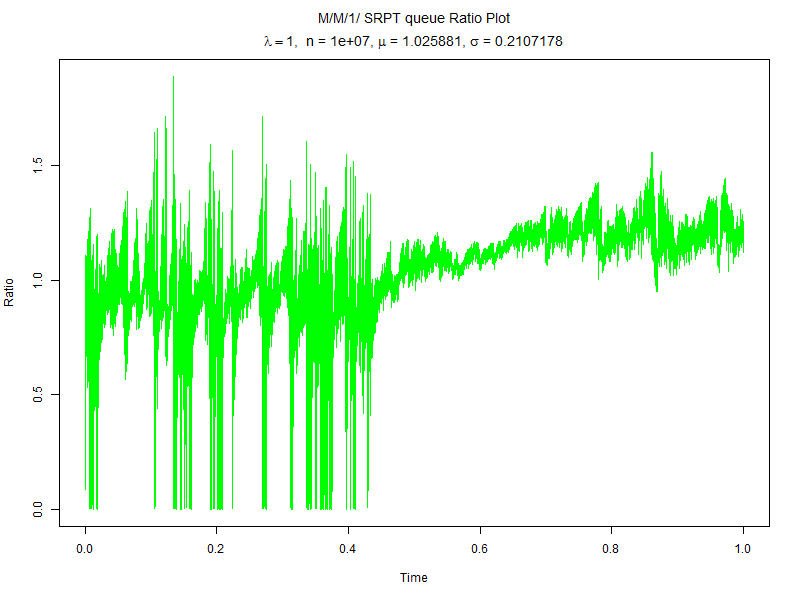
\includegraphics[width = 16cm]{Pictures/ratio1.png}
\vspace{\baselineskip}
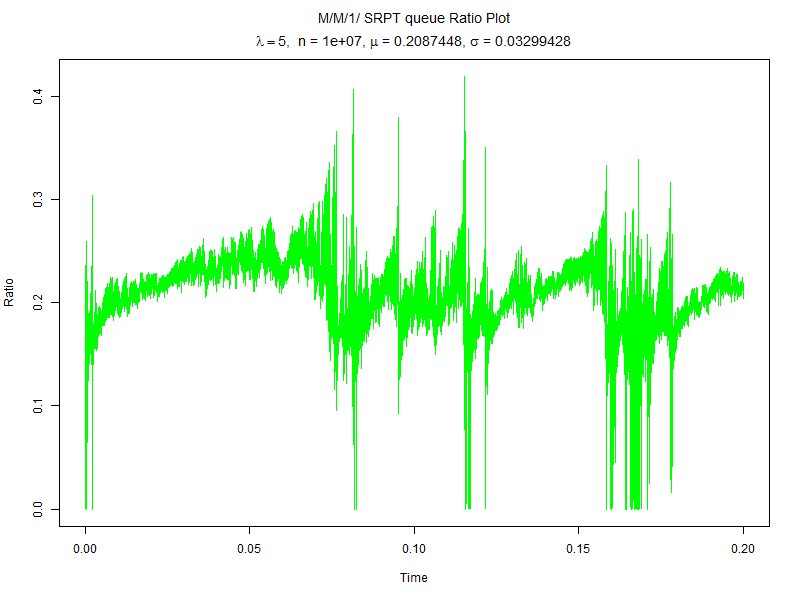
\includegraphics[width=16cm]{Pictures/ratio5.png}
\vspace{\baselineskip}
{\large Plot Characteristics}
\begin{itemize}
\item Relatively Flat
\item Bit of randomness
\item Fluctuates about the line $y=1/\lambda$
\end{itemize}
\vspace{\baselineskip}
\end{minipage}
\quad
\begin{minipage}[t]{16cm}
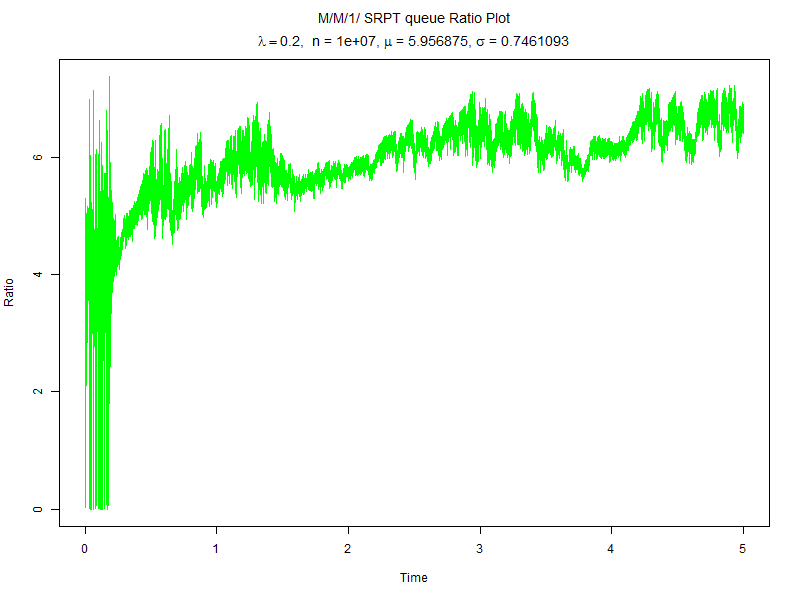
\includegraphics[width=16cm]{Pictures/ratio02.png}
\vspace{\baselineskip}
{\footnotesize
\begin{tabular}{| >{\centering\arraybackslash}m{5cm} | >{\centering\arraybackslash}m{5cm} | >{\centering\arraybackslash}m{5cm} |}
\hline
\multicolumn{3}{ | p{15cm} | } {Table of $\Wfhat/\Qftild$, with $n = 10^{6}$ and $t \in [0,1/\lambda]$}\\
\hline \hline
$\lambda$ & $1/\mu$ & $\sigma$\\
\hline
0.1 & 0.105 & 2.584\\
0.5 & 0.505 & 0.363\\
0.7 & 0.658 & 0.248\\
1 & 0.870 & 0.155\\
2 & 1.972 & 0.092\\
5 & 5.028 & 0.041\\
13 & 13.024 & 0.014\\
\hline
\end{tabular}}
\vspace{2.5\baselineskip}

{\large Table Charterisitics}
\begin{itemize}
\item $1/\mu \approx \lambda$
\item Large $\sigma$ for $\lambda = 0.1$
\item $\sigma$ tends to decrease as $\lambda$ increases
\end{itemize}
\end{minipage}
\vspace{\baselineskip}

{\bf Prediction}: ${\color{orange}C=\lambda}$
\end{block}
\vspace{\baselineskip}

\begin{block}{\huge Investigating the Prediction {\color{orange} \emph{C } $=\lambda$}}
We now display graphics of the rescaled workload ${\color{orange}\lambda}{\color{red}\What}$ and rescaled queue length ${\color{green}\Qtild}$ processes for $n=10^7$ and $t \in [0,1/\lambda]$.
\vspace{\baselineskip}

\begin{minipage}[t]{17cm}
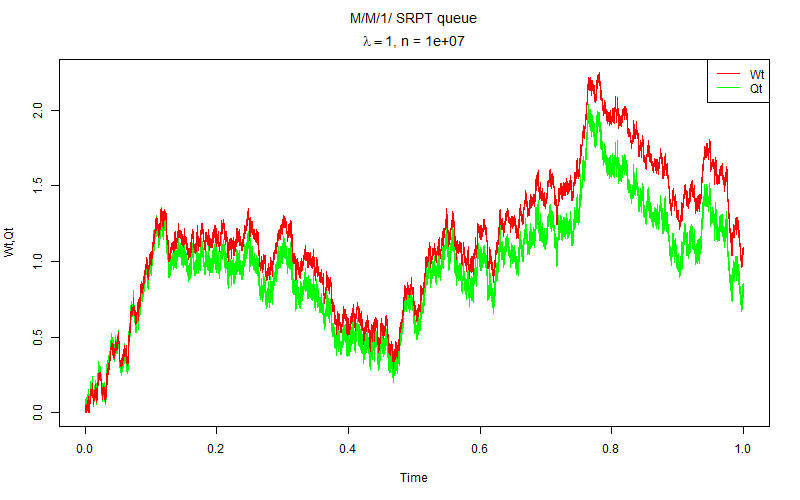
\includegraphics[width = 17cm]{Pictures/normalPlot1_2.png}
\end{minipage}
\begin{minipage}[t]{17cm}
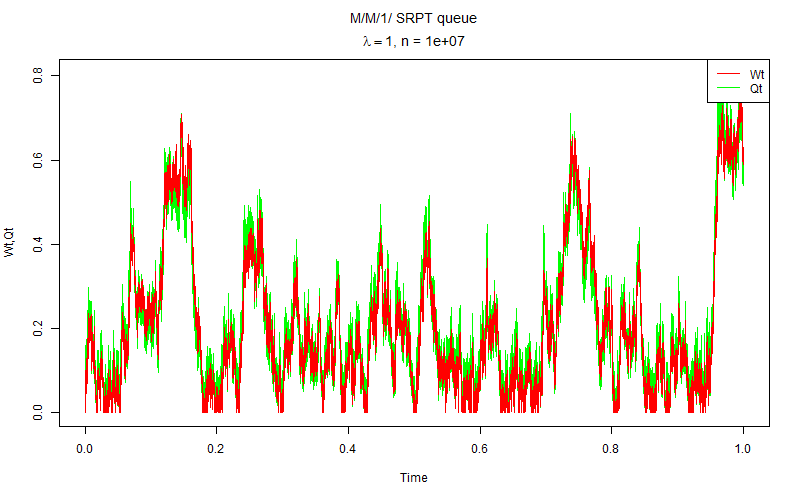
\includegraphics[width = 17cm]{Pictures/normalPlot1_1.png}
\end{minipage}
{\large Plot Characteristics for $\lambda=1$}\\
\begin{itemize}
\item Processes are relatively close throughout
\item As rescaled workload increases, it often slightly exceed rescaled queue length, as on the left
\item Rescaled processes are often very close and frequently zero, as on the right
\item Mimics outcome of Hunsperger and Puha `12, where only ${\color{orange}\lambda}=1$ was considered.
\end{itemize}
\end{block}

\end{textblock}







\begin{textblock}{35}(80,7)
\begin{block}{\huge More Detailed Examination of the Error}
%Again we plot the two processes {\color{red} $\What$ in red} and {\color{green} $\Qtild$ in blue}.
Here we demonstrate that plots for other values of ${\color{orange}\lambda}$ have similar
characteristics.  Also, to more effectively show how close the two processes are,
we plot the difference between the two processes, which we define the error,
{\color{blue}
\[
\error = {\color{orange}\lambda} \Wfhat - \Qftild.
\]
}
We plot {\color{blue}$\error$} in blue in a separate figure on the right,
along with the largest residual service time {\color{red}$R[Qt]$ rescaled by $1/\sqrt{n}$ in red}.
\vspace{\baselineskip}

\begin{minipage}[t]{17cm}
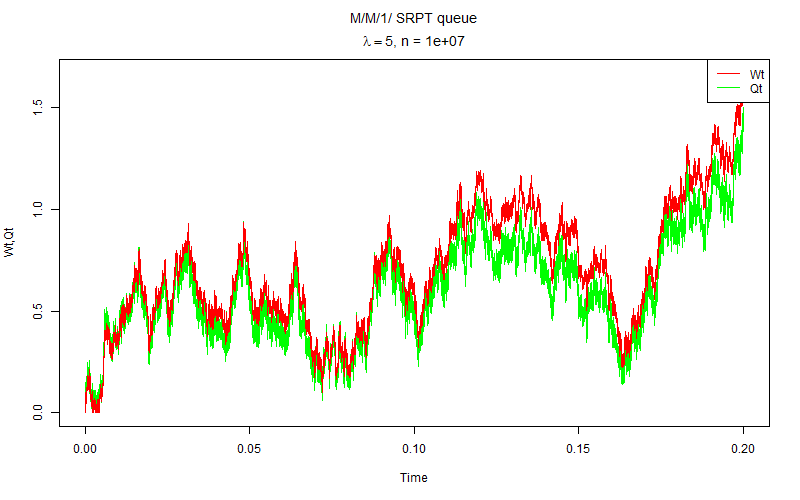
\includegraphics[width=17cm]{Pictures/normalPlot5.png}
\vspace{0.5cm}
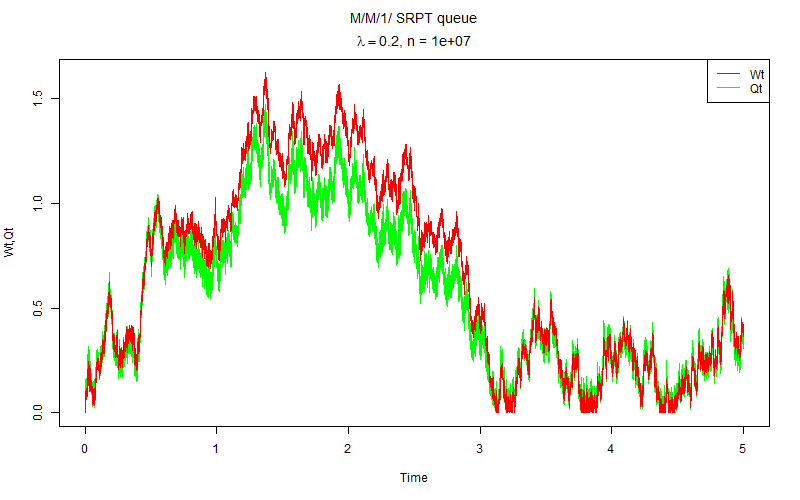
\includegraphics[width=17cm]{Pictures/normalPlot02.png}
\end{minipage}
\begin{minipage}[t]{17cm}
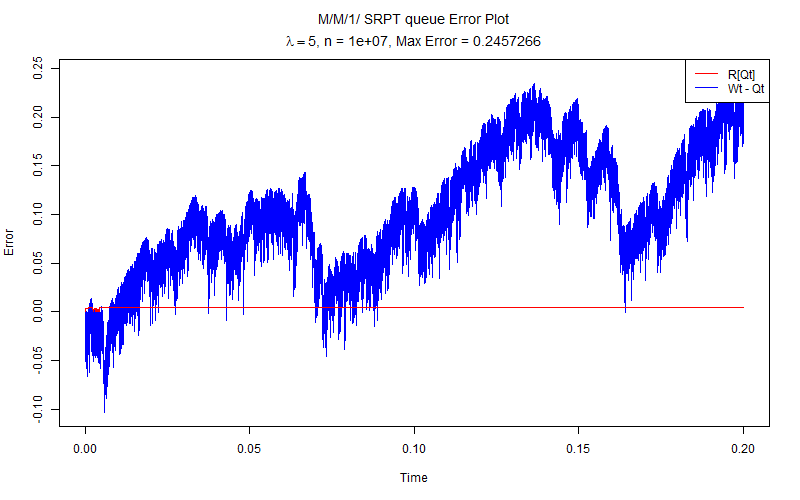
\includegraphics[width=17cm]{Pictures/errorPlot5.png}
\vspace{0.5cm}
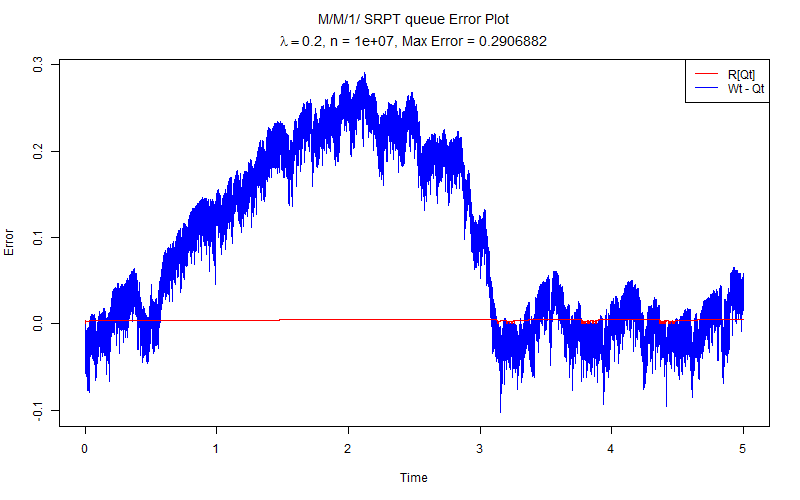
\includegraphics[width=17cm]{Pictures/errorPlot02.png}
\end{minipage}
\vspace{\baselineskip}

{\large Plots of $\lambda = 5$ and $\lambda = 0.2$ with \emph{n }$=10^7$ and \emph{t }$\in [0,1/\lambda]$}
\begin{minipage}[t]{17cm}
\begin{itemize}
\item Closely related processes with varied {\color{orange}$\lambda$}
\item Little separation between processes
\item Supports our claim that {\color{orange}$C=\lambda$}
\end{itemize}
\end{minipage}
\begin{minipage}[t]{17cm}
\begin{itemize}
\item Largest errors typically above the \emph{y}-axis
\item Error plots are similarly shaped
\item Maximum errors are similar size
\end{itemize}
\end{minipage}
\end{block}
%\vspace{\baselineskip}

\begin{block}{\huge  Large \emph{n} Simulations}
We created new code to handle larger values of $n$, in which we track the maximum error defined as
\[
M = \max_{t\in[0,1]} \left | \lambda \What - \Qtild \right |.
\]
\begin{center}
{\footnotesize note we have a new time interval [0,1]}
\end{center}

In our tables, $\mu$ is the average of $M$ over our samples and $\sigma$ is the sample standard deviation. $P(M \leq x)$ denotes the probability that $M$ is less than or equal to $x$

\begin{minipage}[t]{18cm}
{\small
\begin{tabular}[t]{ | >{\centering\arraybackslash}m{5cm} | >{\centering\arraybackslash}m{2.5cm} | >{\centering\arraybackslash}m{2.5cm} | >{\centering\arraybackslash}m{2.5cm} | >{\centering\arraybackslash}m{2.5cm} |}
\hline
\multicolumn{5}{| c |}{$\lambda = 1$ Unbiased Estimators}\\
\hline \hline
\multicolumn{1}{| c |}{Sample Size} & 100 & 100 & 100 & 25\\ \hline
\multicolumn{1}{| c |}{$n$} & $10^{5}$ & $10^{6}$ & $10^{7}$ & $10^{8}$\\ \hline
\multicolumn{1}{| c |}{$\mu$} & 0.347 & 0.309 & 0.301 & 0.270\\ \hline
\multicolumn{1}{| c |}{$\sigma$} &	0.143 & 0.140 & 0.150 & 0.129\\ \hline
$P(M \leq 0.1)$ & 0 & 0 & 0.01 & 0.04\\
%$P(M \leq 0.15)$ & 0 & 0.03 & 0.17 & 0.16\\
$P(M \leq 0.2)$	& 0 & 0.31 & 0.31 & 0.4\\
%$P(M \leq 0.25)$ & 0.28 & 0.41	 & 0.46 & 0.56\\
$P(M \leq 0.3)$	& 0.52 & 0.54 & 0.56 & 0.64\\
%$P(M \leq 0.35)$ & 0.63 & 0.69 & 0.67 & 0.76\\
$P(M \leq 0.4)$	& 0.77 & 0.76 & 0.73 & 0.84\\
%$P(M \leq 0.45)$ & 0.83 & 0.84 & 0.79 & 0.88\\
$P(M \leq 0.5)$	& 0.88 & 0.88 & 0.85 & 0.96\\
\hline
\end{tabular}
}
\end{minipage}
\begin{minipage}[t]{16cm}
{\small
\begin{tabular}[t]{| >{\centering\arraybackslash}m{5cm} | >{\centering\arraybackslash}m{2.5cm} | >{\centering\arraybackslash}m{2.5cm} | >{\centering\arraybackslash}m{2.5cm} |}
\hline
\multicolumn{4}{| c |}{$\lambda = 5$ Unbiased Estimators}\\
\hline \hline
\multicolumn{1}{| c |}{Sample Size} & 100 & 100 & 100 \\ \hline
\multicolumn{1}{| c |}{$n$} & $10^{5}$ & $10^{6}$ & $10^{7}$\\ \hline
\multicolumn{1}{| c |}{$\mu$} & 1.091 & 0.935 & 0.870\\ \hline
\multicolumn{1}{| c |}{$\sigma$} & 0.465 & 0.412 & 0.435\\ \hline
$P(M\leq .2)$&0&0&0\\
%$P(M\leq.3)$&0&0.02&0.01\\
$P(M\leq.4)$&0.05&0.05&0.09\\
%$P(M\leq.5)$&0.08&0.11&0.17\\
$P(M\leq.6)$&0.16&0.25&0.31\\
%$P(M\leq.7)$&0.18&0.35&0.41\\
$P(M\leq.8)$&0.28&0.41&0.55\\
%$P(M\leq.9)$&0.4&0.49&0.66\\
$P(M\leq1)$&0.49&0.6&0.73\\
%$P(M\leq1.1)$&0.55&0.74&0.77\\
$P(M\leq1.2)$&0.61&0.79&0.79\\
%$P(M\leq1.3)$&0.68&0.82&0.83\\
\hline
\end{tabular}
}
\end{minipage}

\begin{minipage}[t]{18cm}
{\small
\begin{tabular}[t]{ | >{\centering\arraybackslash}m{5cm} | >{\centering\arraybackslash}m{2.5cm} | >{\centering\arraybackslash}m{2.5cm} | >{\centering\arraybackslash}m{2.5cm} | >{\centering\arraybackslash}m{2.5cm} |}
\hline
\multicolumn{5}{| c |}{$\lambda = 0.2$ Unbiased Estimators}\\
\hline \hline
\multicolumn{1}{| c |}{Sample Size} & 100 & 100 & 100 & 25\\ \hline
\multicolumn{1}{| c |}{$n$} & $10^{5}$ & $10^{6}$ & $10^{7}$ & $10^{8}$\\ \hline
\multicolumn{1}{| c |}{$\mu$} & 0.211 & 0.149 & 0.107 & 0.086\\ \hline
\multicolumn{1}{| c |}{$\sigma$} & 0.031 & 0.023 & 0.020 & 0.026\\ \hline
$P(M\leq.05)$	&0	&0	&0	&0\\
$P(M\leq.1)$	&0	&0	&0.39	&0.8\\
$P(M\leq.15)$&0	&0.57	&0.96	&0.96\\
$P(M\leq.2)$ & 0.43 	&0.97	&1	&1\\
\hline
\end{tabular}
}
\end{minipage}
\begin{minipage}[t]{16cm}
\vspace{1cm}
{\large Table Characteristics}
\begin{itemize}
\item $\mu$ decreases as $n$ increases
\item $\sigma$ seems to slowly decrease
\item $P(M \leq x)$ generally increases as $n$ increases
\item Supports that $M$ tends to zero, but seems to do so more slowly for larger ${\color{orange}\lambda}$
\item Additional evidence supporting ``Suspected Behavior" and Conjecture, i.e., the correction factor ${\color{green}\ln(\sqrt{n})}$ and constant {\color{orange}$C = \lambda$}
\end{itemize}
\end{minipage}

\end{block}
\end{textblock}


\end{frame}
\end{document}
